\documentclass[wide,a4paper,titlepage,12pt] {article}
\usepackage{polski}
\usepackage[utf8]{inputenc}
\usepackage{listings}
\usepackage{slashbox}
\usepackage[table]{xcolor}
\usepackage{graphicx,pdflscape}
\usepackage{placeins}


\title{Grafika komputerowa}
\author{Tymon Tobolski (181037)}

% Title page layout (fold)
\makeatletter
\renewcommand{\maketitle}{
\begin{titlepage}
  \begin{center}
    \vspace*{3cm}
    \LARGE \@title \par
    \vspace{2cm}
    \textit{\small Autor:}\par
    \normalsize \@author\par \normalsize
    \vspace{3cm}
    \textit{\small Prowadzący:}\par
    Dr inż. Tomasz Kapłon \par
    \vspace{2cm}
    Wydział Elektroniki\\ III rok\\ Pn TP 08.15 - 11.00\par
    \vspace{4cm}
    \small 14 listopada 2011
  \end{center}
\end{titlepage}
}
\makeatother
  \lstset{
    language=c++,
    basicstyle=\ttfamily\scriptsize,
    numbers=left,
    numberstyle=\scriptsize,
    stepnumber=10,
    numbersep=9pt,
    showspaces=false,
    showstringspaces=false,
    showtabs=false,
    breaklines=true,
  }

\begin{document}
\maketitle
  \section{Cel laboratorium}
  \paragraph{}
  Celem laboratorium było zapoznanie sie z modeownaiem obiektów w przestrzeni trójwymiarowej.
  Głownym zadaniem było narysowanie modelu jajka na podstawie podanych wzorów transformacji.

  \section{Jajko}
  \paragraph{}
  Program rysuje model jajka w trzech wersjach
  \begin{itemize}
    \item pojedyncze punkty
    \item siatka
    \item kolorowe jajko złożone z trójkątów
  \end{itemize}

  \subsection{Generowanie punktów w przestrzeni 3D}
  \paragraph{}
  \lstinputlisting{calc.cpp}

  \subsection{Reprezentacja punktowa}
  \paragraph{}

  \lstinputlisting{points.cpp}

  \begin{figure}[htbp]
    \begin{center}
      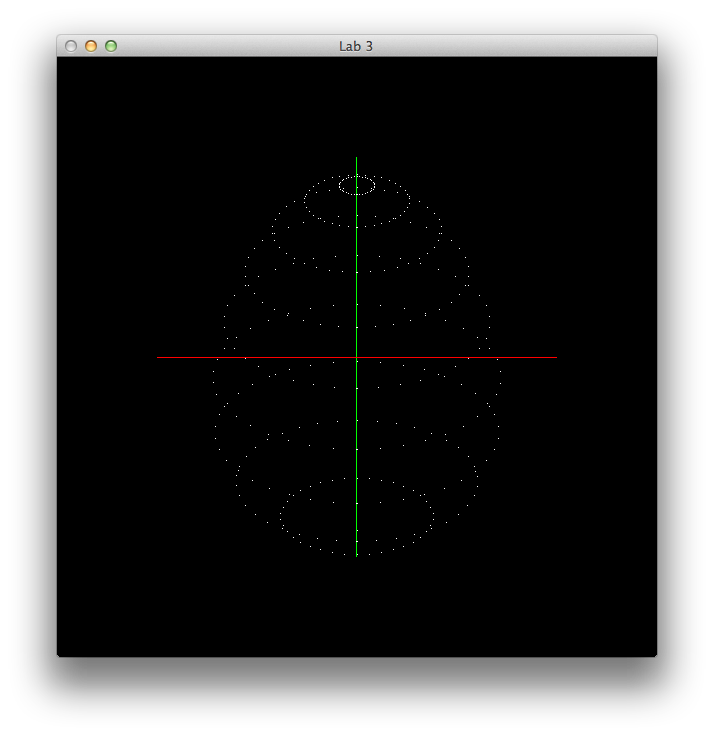
\includegraphics[scale=0.6]{points.png}
      \caption{Reprezentacja punktowa}
    \end{center}
  \end{figure}

  \newpage


  \subsection{Siatka}
  \paragraph{}

  \lstinputlisting{mesh.cpp}

  \begin{figure}[htbp]
    \begin{center}
      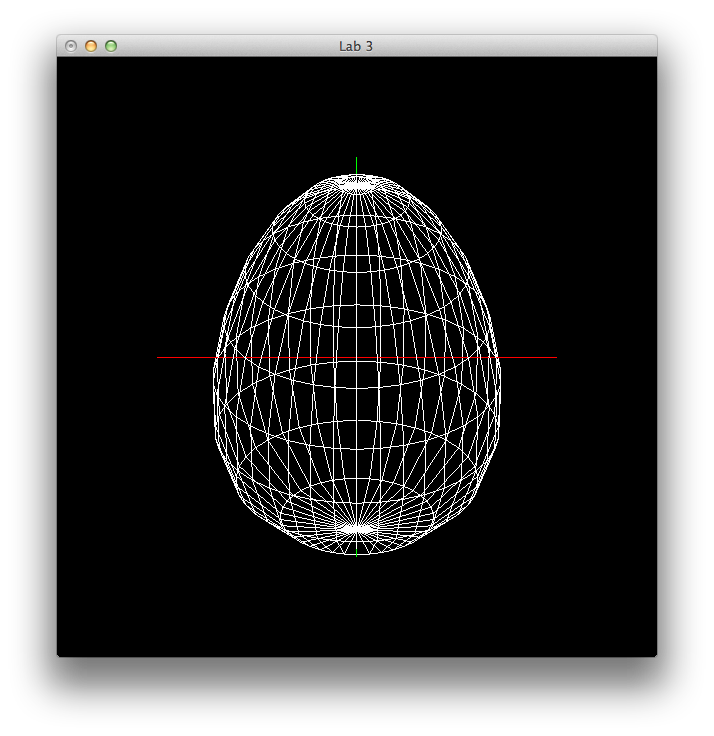
\includegraphics[scale=0.6]{mesh.png}
      \caption{Siatka}
    \end{center}
  \end{figure}

  \newpage


  \subsection{Pełne, kolorowe jajko}
  \paragraph{}

  \lstinputlisting{fill.cpp}

  \begin{figure}[htbp]
    \begin{center}
      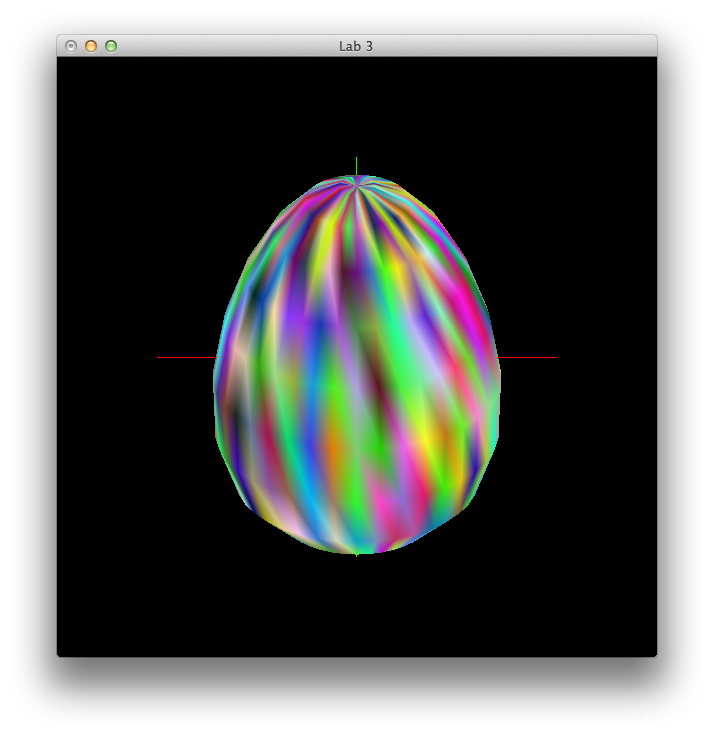
\includegraphics[scale=0.6]{fill.png}
      \caption{Pełne, kolorowe jajko}
    \end{center}
  \end{figure}

  \newpage


  \subsection{Usunięcie "szwu"}
  \paragraph{}
  Przy kolorowym jajku występował problem tzw. "szwu" - widocznej lini łączącej dwie połowy obiektu.
  Rozwiązaniem na to było ustawienie takich samych kolorów dla punktów leżących obok siebie.

  \lstinputlisting{colors.cpp}


  \section{Wnioski}
  \paragraph{}
  Po ustaleniu które punkty należy ze sobą połączyc aby uzyskać pełne, kolorowe jajko jedynym problemem
  pozostał wspomniany "szew". Udało się go wyeliminować ustalając kolory odpowiednich punktów.
  Poziom przybliżenia powstałych krawędzi i płaszczyzn do prawdziwego jajka zależy od parametru $N$ - ilości punktów z których składa sie wygenerowany obiekt.

\end{document}